\documentclass{standalone}

\begin{document}
\chapter*{Introduction}\addcontentsline{toc}{chapter}{Introduction}
\markboth{INTRODUCTION}{}

Colorectal cancer is a malignant neoplasm of the large intestine resulting from the uncontrolled proliferation of the cells making up the colorectal tract.
Colorectal cancer is the second malignant tumor per number of deaths after the lung cancer and the third for number of new cases after the breast and lung cancer\cite{cancerstats}.\\
Among the risk factors for this kind of cancer, non hereditary could range from colon polyps to long-standing ulcerative colitis, from Crohn's disease to old age. 
Also genetic history (HNPCC or Lynch syndrome) and nutritional factors as diabetes II can increase the probability of develop cancer \cite{tesicoppola}.
Preventive measures for colorectal cancer include physical activity, reducing the consumption of processed meat and alcohol, and avoiding smoking\cite{stats2019}.
\begin{figure}[h!]
	\centering
	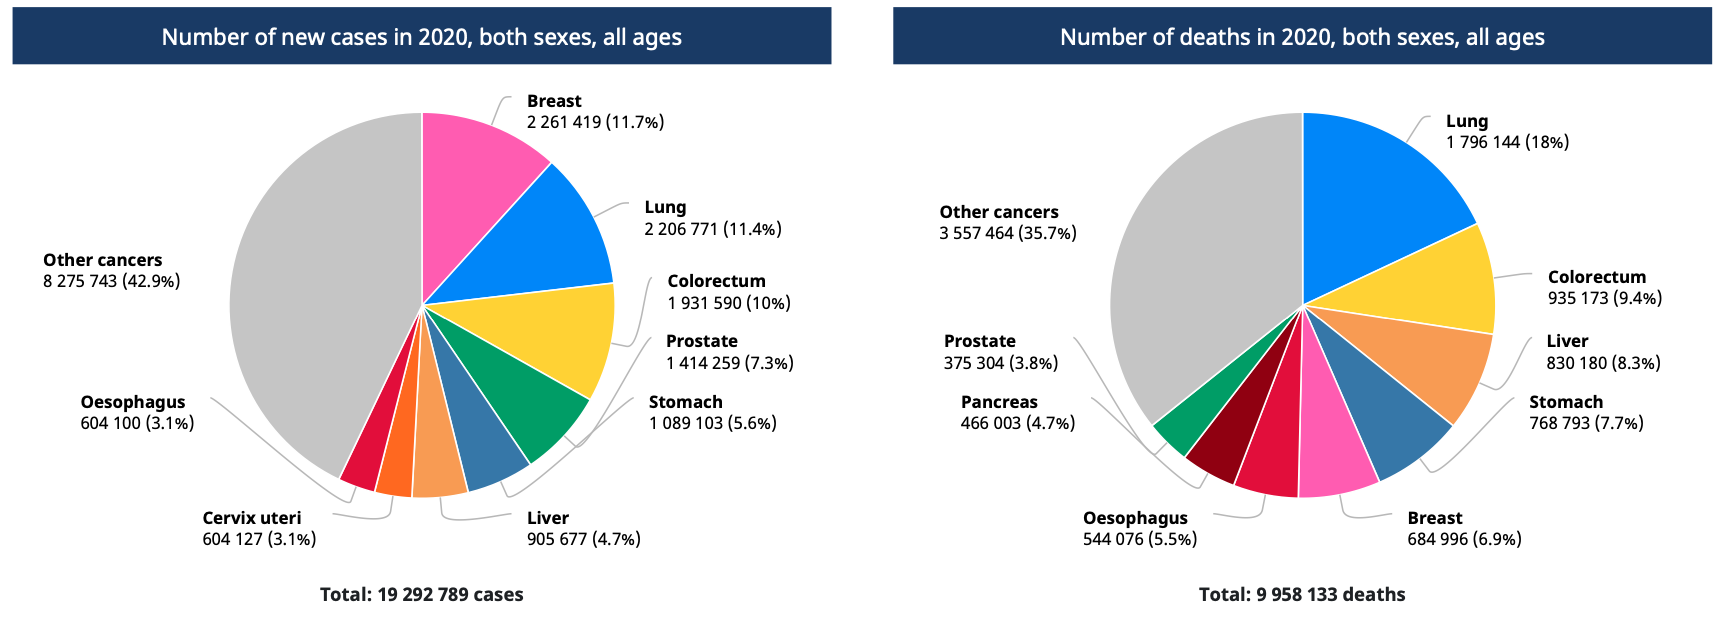
\includegraphics[width=\linewidth]{../images/cancerstats.png}
	\caption{World's cancer cases and deaths. From \cite{cancerstats} }
\end{figure}
\\
Screening and diagnosis methods for colorectal cancer can be based on different techniques. 
The gold standard in medical routines is colonoscopy which is an invasive technique\cite{jovana}.
Among medical imaging techniques, Magnetic Resonance Imaging (MRI) and Computed Tomography (CT) are the most used\cite{tesicoppola}. 
In particular Magnetic Resonance Imaging (MRI) is used for pre-operative predictions and for the evaluation of the neo-adjuvant therapy of patients affected by colorectal cancer \cite{tesicoppola}.

\begin{figure}[htp]

    \centering
    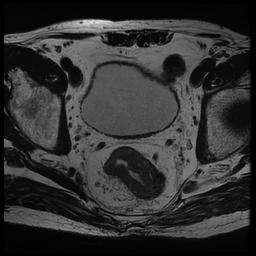
\includegraphics[width=.3\textwidth]{../images/T2AX_Alta_8.png}\hfill
    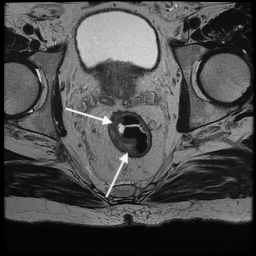
\includegraphics[width=.3\textwidth]{../images/T2AX_BO11_5.png}\hfill
    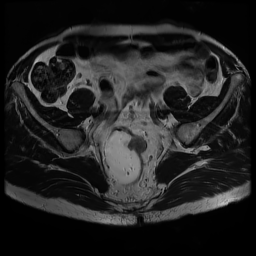
\includegraphics[width=.3\textwidth]{../images/T2AX_BO1_9.png}
    
    \caption{Example of MRI scans of patients affected by colorectal cancer. From Sant'Orsola original Dataset.}
    \label{trittico}
    
    \end{figure}
In order to get information about diagnosis, therapy evaluation, stage of colorectal cancer, analysis on radiological images can be performed through the application of dedicated algorithms.\\
In this scenario, the correct and fast identification of the cancer regions is a fundamental task. 
Up to now, this segmentation task is performed using manual or semi-automatic techniques, which are time-consuming (requiring hours per day) and subjected to the operator expertise since it requires the interaction with trained specialists\cite{tesicoppola, jovana}.
Moreover, due to the highly sensitivity to the operator expertise, the  obtained results cannot be reproduced\cite{Trebeschi2017}.
To overcome these issues, an automatic and fast way is required.\\
The aim of this project is to provide an automated pipeline to predict the response to neo-adjuvant chemo-radiotherapy of patients affect by colorectal cancer. 
The work is based and tested on MRI scans provided by IRCCS Sant’Orsola-Malpighi Policlinic.\\
The discussion will start focusing on medical digital images to understand their properties and features.
After that, an overview on the main segmentation method for the identification of the cancer regions will be given.
Then, the main pipeline characteristics and structure will be described.
In particular, how the segmentation was achieved using a Convolutional Neural Network and how extracting and processing medical image features.
Finally, the result will be shown and discussed.





\end{document}